\documentclass[a4paper,12pt]{article} 


\usepackage[T2A]{fontenc}			% кодировка
\usepackage[utf8]{inputenc}			% кодировка исходного текста
\usepackage[english,russian]{babel}	% локализация и переносы


% Математика
\usepackage{amsmath,amsfonts,amssymb,amsthm,mathtools} 

\usepackage{gensymb}	
\usepackage{wasysym}

% Картинки
\usepackage{graphicx}
\graphicspath{{images/}}

%Заговолок
\usepackage[left=2cm,right=2cm,
    top=2cm,bottom=2cm,bindingoffset=0cm]{geometry}

\usepackage{titling}


\author{Петров Артём Антонович, группа 721}
\title{Лабораторная работа № 3.2.6 "Исследование гальванометра"}
\date{\today}

\begin{document} % начало документа

\begin{minipage}[t][7cm]{\textwidth}
\maketitle
\end{minipage}


%\subsection*{Теоретическое введение}
%\bigskip
%Сила тока, протекающего через гальванометр в стационарном режиме:
%   \begin{equation}
%   \label{fl.1}
%   I = U_0 \frac{R_1}{R_2}\frac{1}{R + R_0}.
%   \end{equation}
%   Динамическая постоянная:
%   \begin{equation}
%   \label{fl.2}
%   C_I = \frac{I}{\varphi} = \frac{2aI}{x}, \quad \sigma_{C_I} = \sqrt{\left( \frac{I}{x}\sigma_{2a} \right)^2 + \left( 2a \sigma_{\frac{I}{x}} \right)^2}.
%   \end{equation}
%   Логарифмический декремент затухания:
%   \begin{equation}
%   \label{fl.3}
%   \Theta = \ln \frac{x_n}{x_{n + 1}}, \quad \sigma_\Theta = \sqrt{\left(\frac{\sigma_{x_n}}{x_n}\right)^2 + \left( \frac{\sigma_{x_{n + 1}}}{x_{n + 1}} \right)^2}.
%   \end{equation}
%   Критическое сопротивление ($X = (R_0 + R)^2$, $Y = 1 / \Theta^2$):
%   \begin{equation}
%   \label{fl.4}
%   R_{\text{кр}} = \frac{1}{2\pi}\sqrt{\frac{\Delta X}{\Delta Y}} - R_0, \quad \sigma_{R_\text{кр}} = \frac{1}{4\pi} \sqrt{\frac{\Delta Y}{\Delta X}} \cdot \sigma_{\frac{\Delta X}{\Delta Y}}.
%   \end{equation}
%   Баллистическая постоянная:
%   \begin{equation}
%   \label{fl.5}
%   C_{Q_\text{кр}} = 2a \frac{R_1}{R_2} \frac{U_0 C}{l_{max}^\text{кр}}
%   \end{equation}

\bigskip

\subsection*{Экспериментальная установка}
\bigskip

Параметры установки: 

собственное сопротивление гальванометра $R_0 = [475 \pm 1] Ohm$,

сопротивление $R_2 = [10,0 \pm 0,1]kOhm $,

ёмкость конденсатора $C = [2,0 \pm 0,1]\mu F $,

напряжение на источнике $U_0 = [2.03 \pm 0.01]V$,

расстояние от зеркальца гальванометра до экрана (и до источника света, соответственно) $a = [136 \pm 1] cm$.

   
   \begin{figure}[h!]
   \centering
   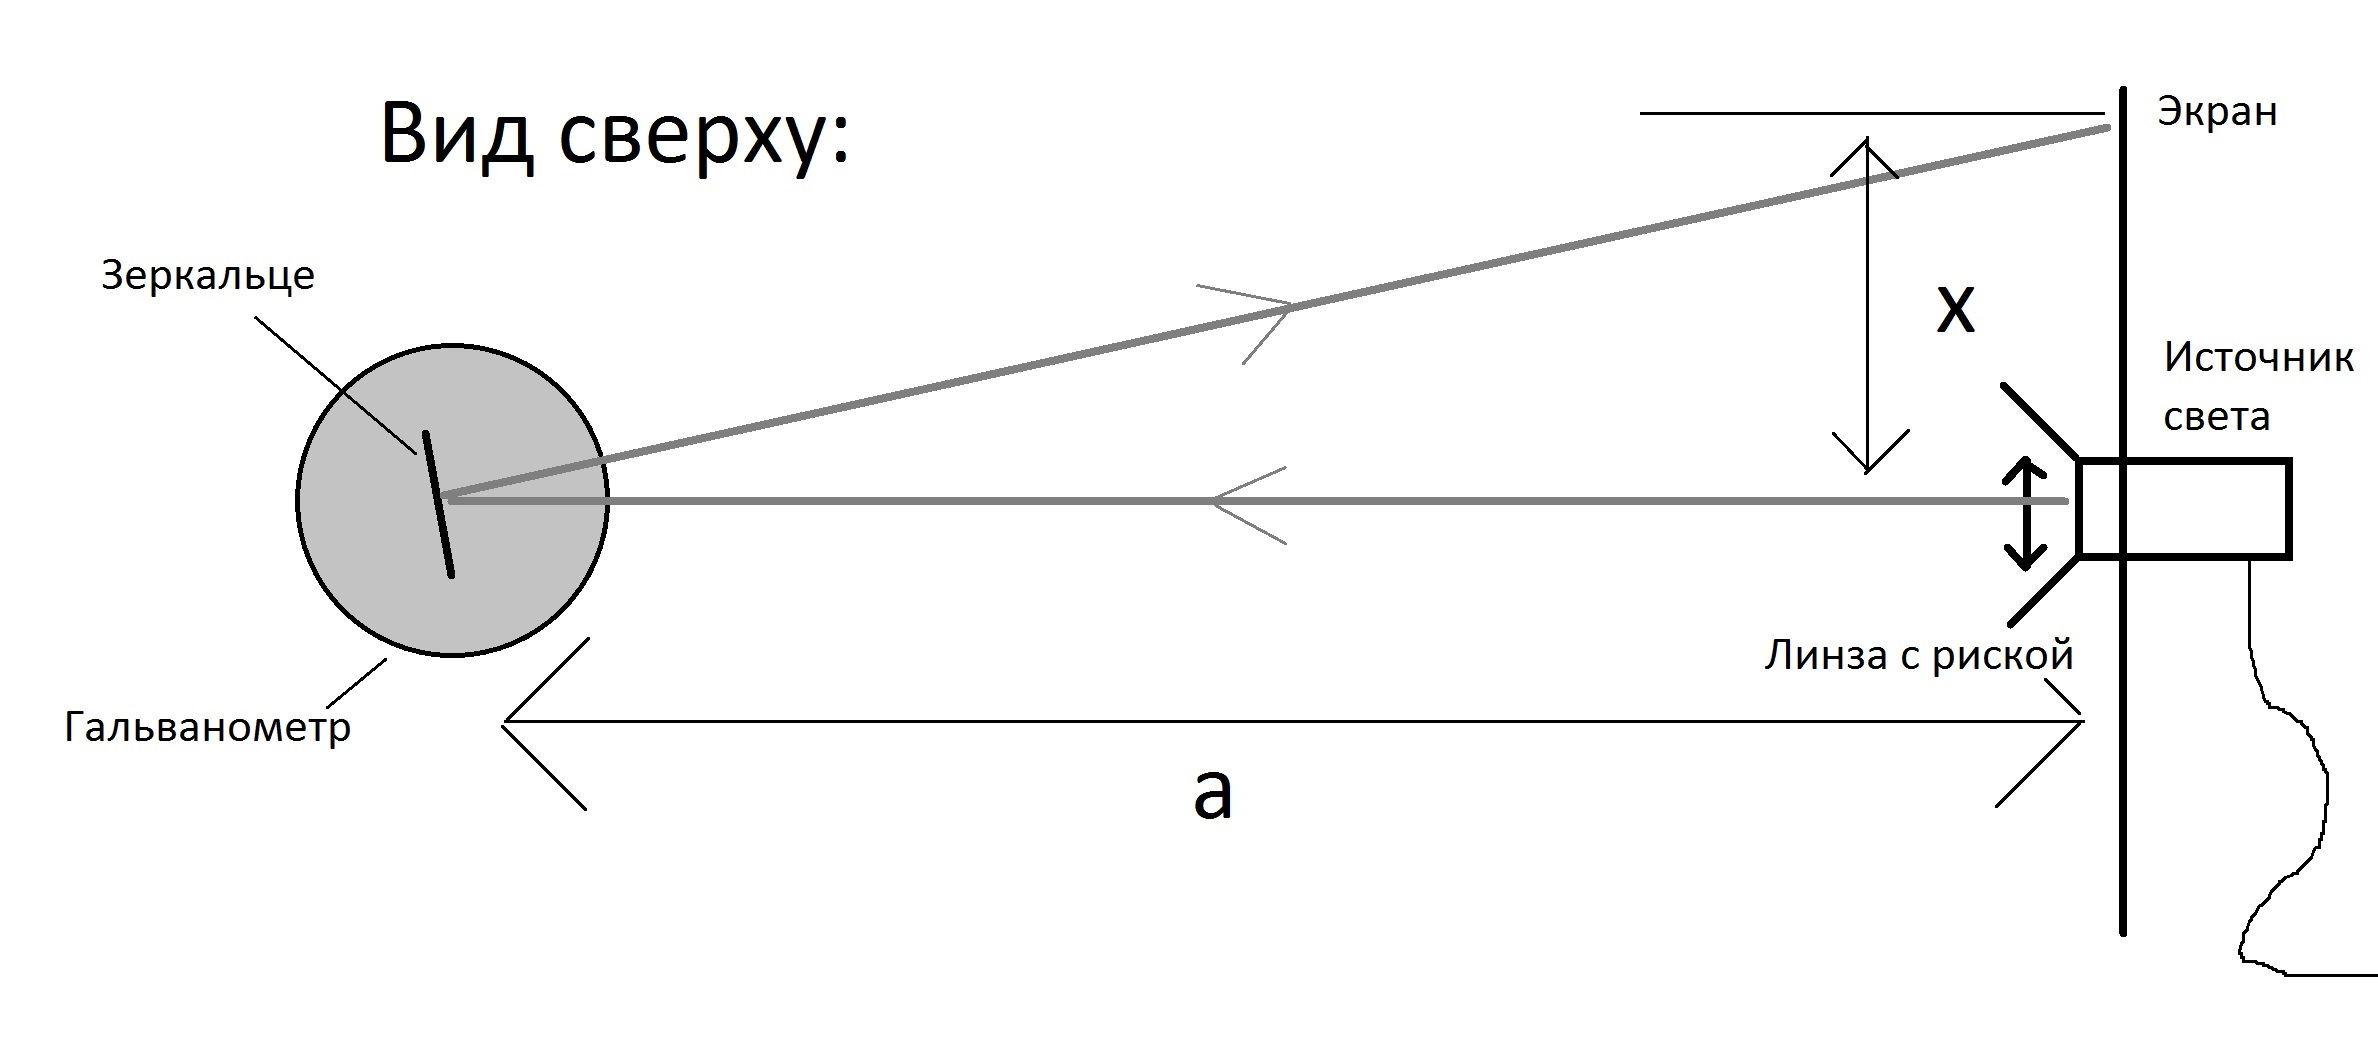
\includegraphics[width=14cm]{fig3.jpg} 
   \caption{Схема установки для измерения отклонения зеркала гальванометра.} 
   \label{fig.3} 
   \end{figure}   
   
   \begin{figure}[h!]
   \centering
   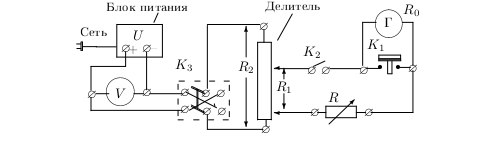
\includegraphics[width=12cm]{fig1.jpg} 
   \caption{Схема установки для работы гальванометра в стационарном режиме.} 
   \label{fig.1} 
   \end{figure}

   \begin{figure}[h]
   \centering
   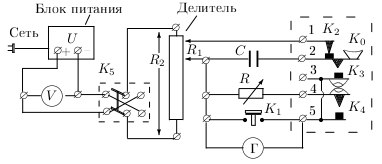
\includegraphics[width=10cm]{fig2.jpg} 
   \caption{Схема установки для определения баллистической постоянной.} 
   \label{fig.2} 
   \end{figure}



\bigskip

\subsection*{Ход работы}
\bigskip

\subsubsection*{Стационарный режим (измерение динамической постоянной)}

Была получена зависимость отклонения зайчика $x$ от сопротивления магазина сопротивлений $R$ при значении входного напряжения $U_0 = [2.03 \pm 0.01] V$, положении делителя $R_1/R_2 = \frac{1}{2000}$. Её можно видеть на графике \ref{PlotA}. Коэффициент наклона графика $\frac{C_1}{2a} = [2,21 \pm 0,05]nA/cm$. Из него мы получаем значение динамической постоянной гальванометра $C_1 = [0.601 \pm 0.14] \mu A$.

   \begin{figure}[h!]
   \centering
   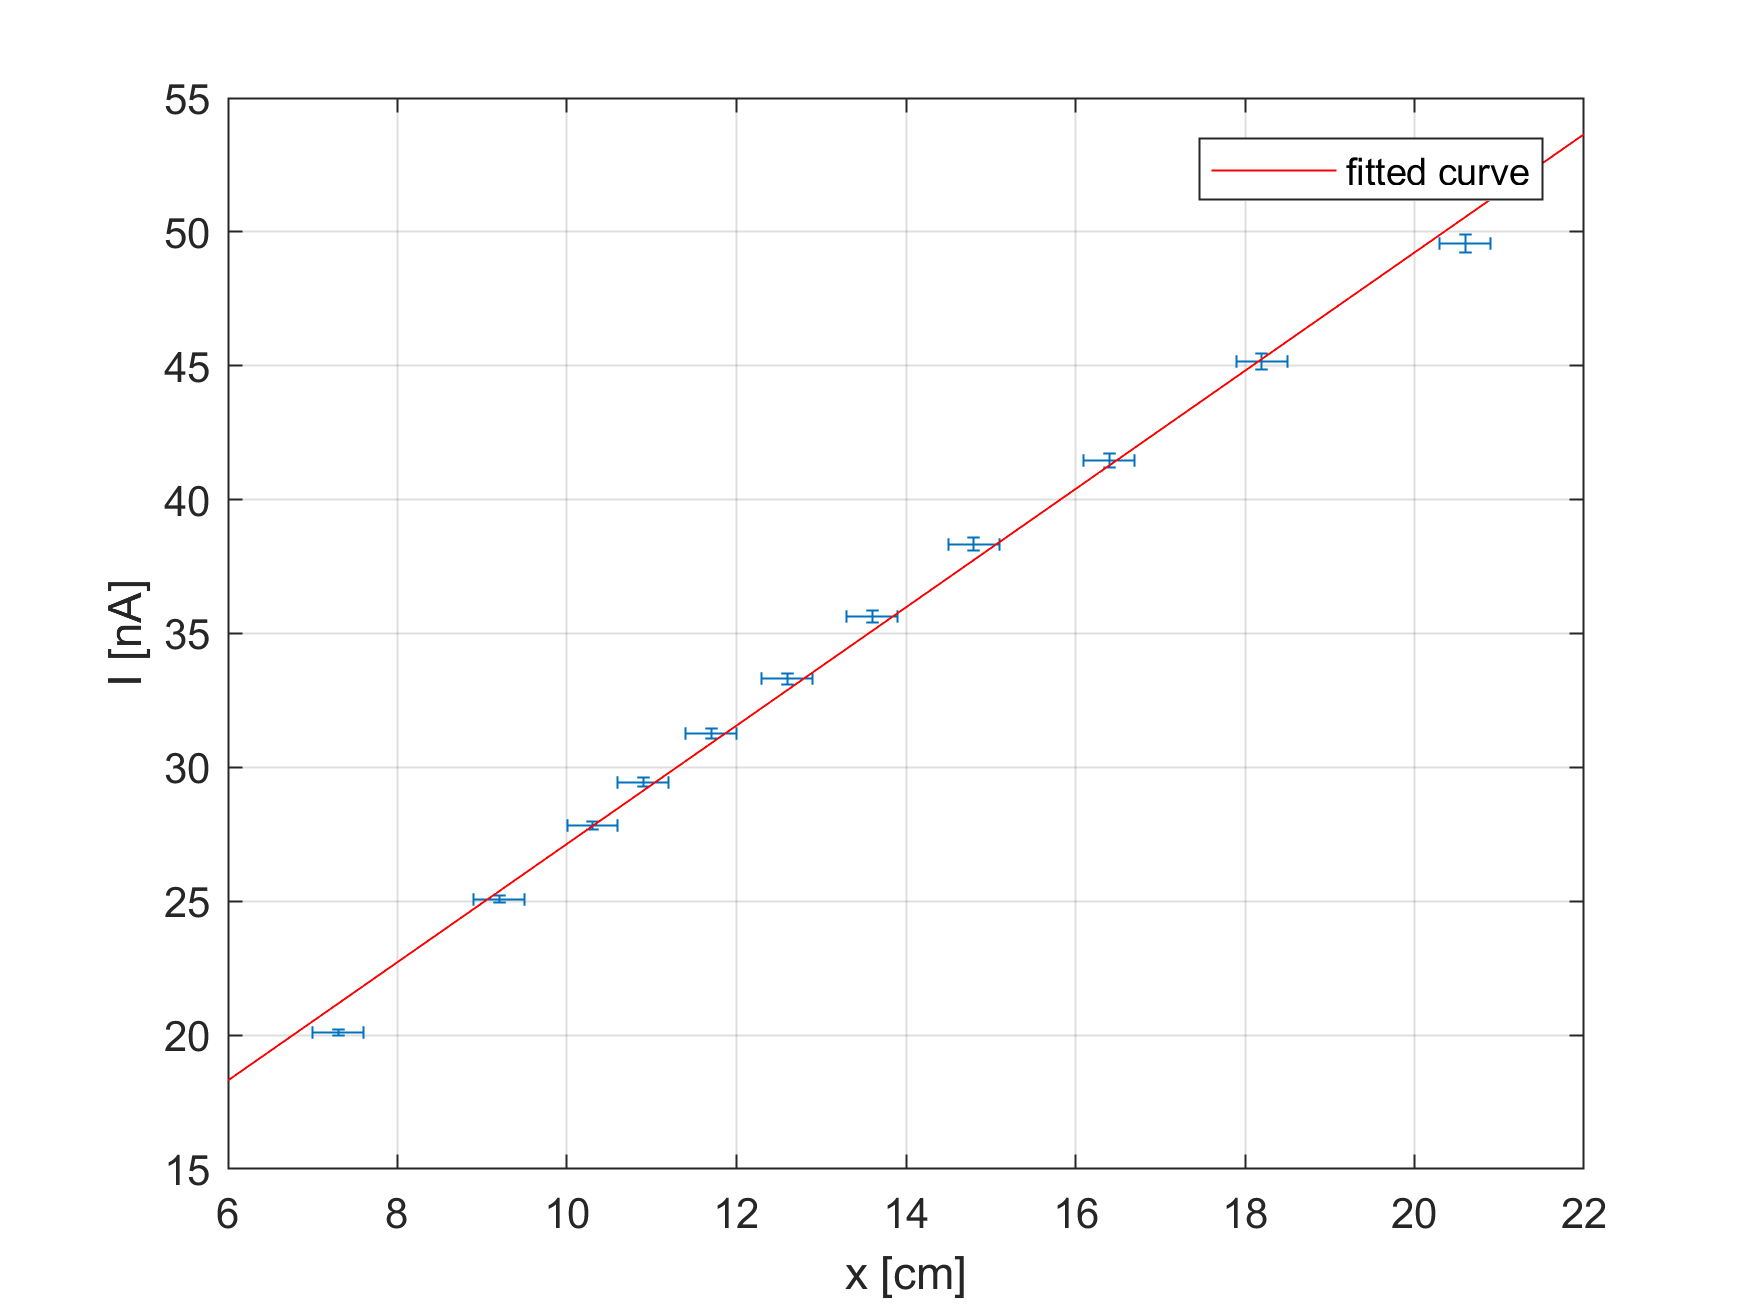
\includegraphics[width=12cm]{PlotA.png} 
   \caption{Зависимость $I(x)$. Коэффициент наклона графика $\frac{C_1}{2a} = [2,21 \pm 0,05]nA/cm$.} 
   \label{PlotA} 
   \end{figure}

\subsubsection*{Стационарный режим (измерение $R_\text{кр}$)}

Для начала был получен логарифмический декремент затухания разомкнутого гальванометра с помощью измерения двух последовательных отклонения зайчика. Получено значение $\theta_0 = [0,307 \pm 0,005]$. Также был измерен период колебаний рамки $T_0 = [6,2 \pm 0,2]sec$.  

Далее было примерно оценено значение $R_\text{кр}$ с помощью наблюдения за тем, при каком R зайчик перестаёт колебаться (начинается "безколебательный" режим). Получено приблизительное значение \textbf{$R_\text{кр} \approx 9.2 kOhm$}.

Далее была получена зависимость $1/\theta^2$ от $(R+R_0)^2$. Её можно видеть на графике \ref{PlotB}. Коэф наклона графика при малых значениях R: $koef = [1,95 \pm 0,18]*10^{-4} kOhm^{-2}$. Откуда получили значение \textbf{$R_\text{кр} = \frac{1}{2\pi}\sqrt{koef^{-1}} - R_0 = [10.9 \pm 0.5] kOhm$}.


\begin{figure}[h!]
   \centering
   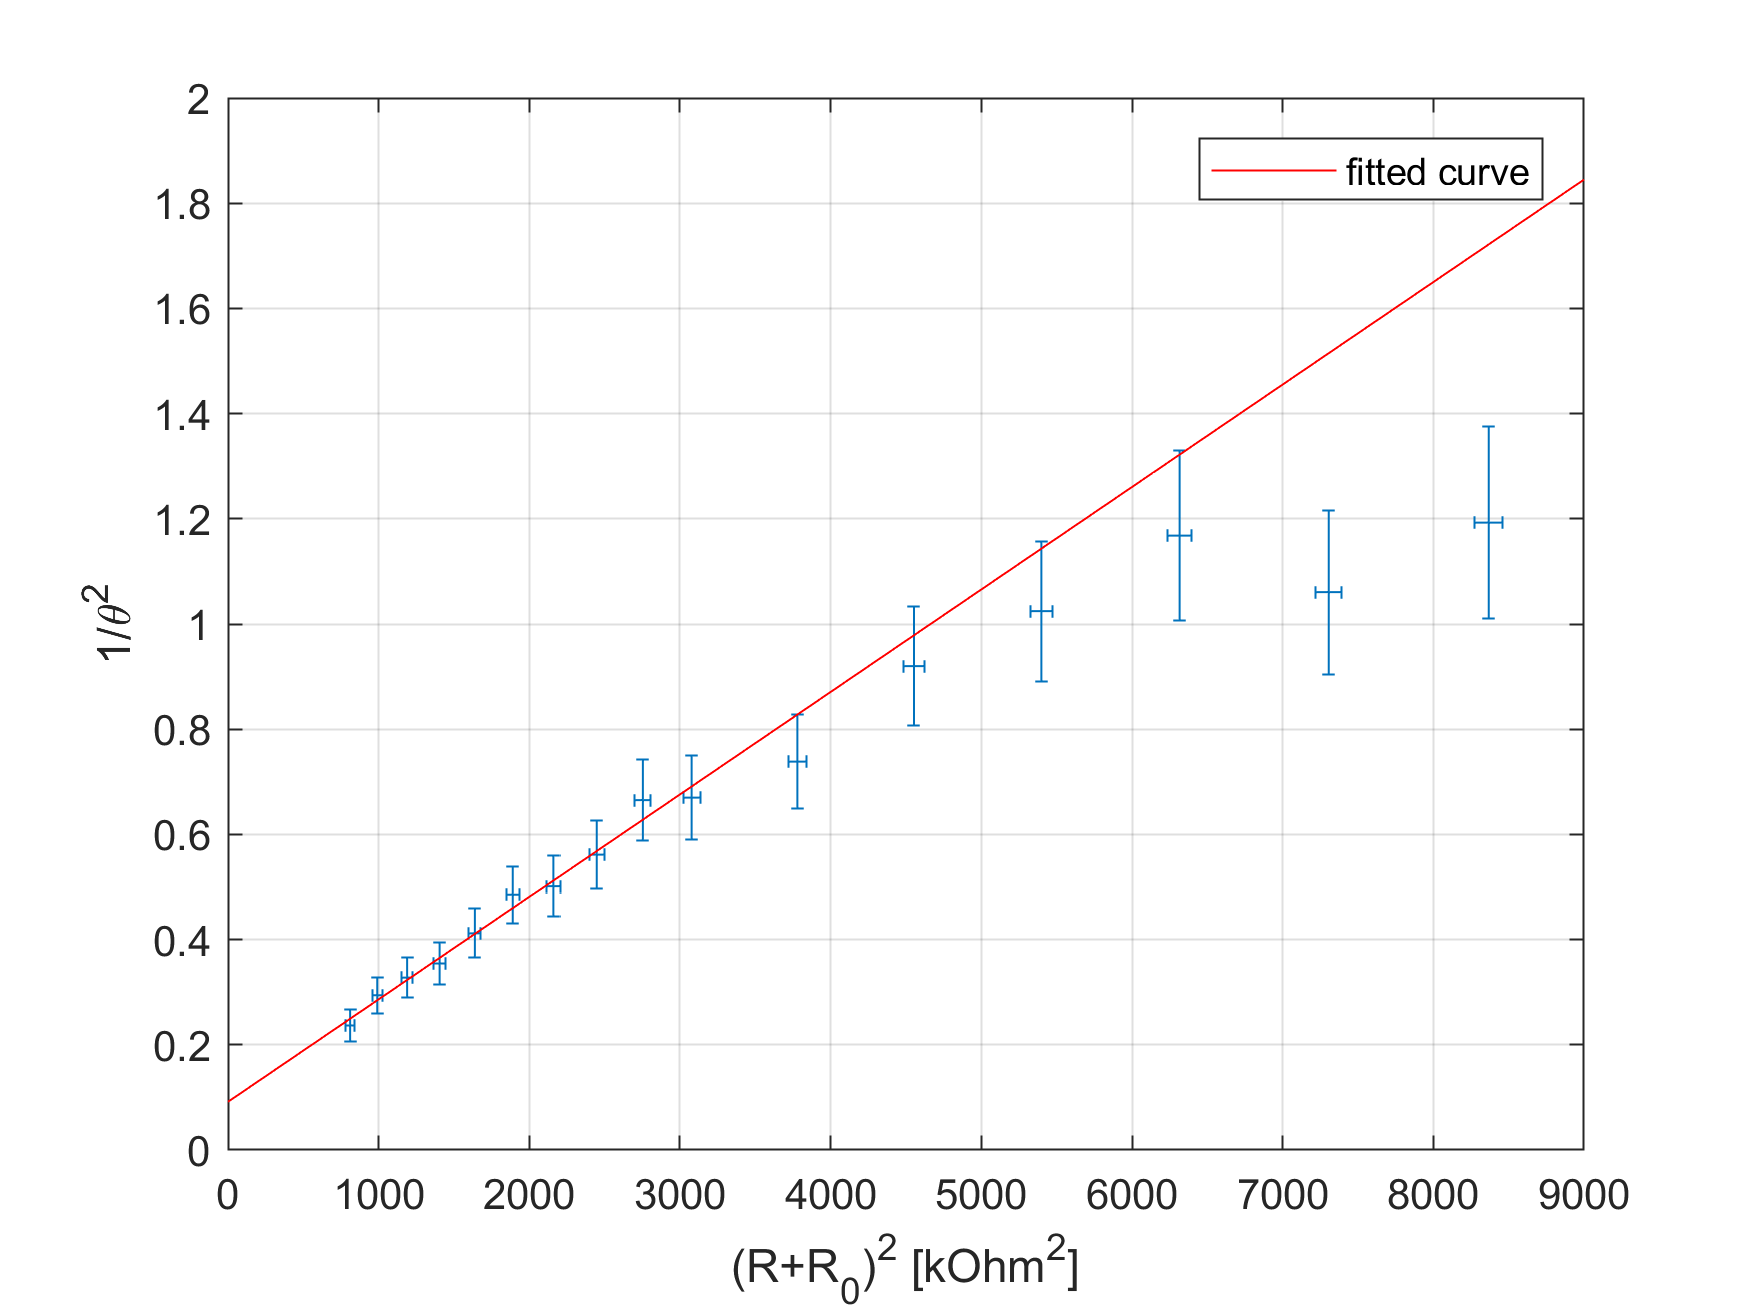
\includegraphics[width=12cm]{PlotB.png} 
   \caption{Зависимость $1/\theta^2$ от $(R+R_0)^2$. Коэф наклона графика при малых значениях R: $koef = [1,95 \pm 0,18]*10^{-4} kOhm^{-2}$} 
   \label{PlotB} 
   \end{figure}
   
\subsubsection*{Баллистический режим (измерение $R_\text{кр}$ и динамической постоянной гальванометра)}
\bigskip

Можно видеть, что время релаксации (время протекания заряда конденсатора через гальванометр) $t = R_0C \approx 10^{-3}sec$ много меньше периода собственных колебаний рамки гальванометра $T_0 = [6,2 \pm 0,2]sec$, а \textbf{значит предложенное в теории приближение, что рамка ускоряется почти мгновенно верно}.

Была получена зависимость максимального отклонения зайчика $l_{max}$ от шунтирующего сопротивления $R$  в баллистическом режиме работы гальванометра (рамка гальванометра разгоняется за счёт заряда, запасённого на конденсаторе за время много меньшее периода его колебаний и затем исследуется движение зайчика на экране). Эту зависимость можно видеть на графике \ref{PlotC}.

\begin{figure}[h!]
   \centering
   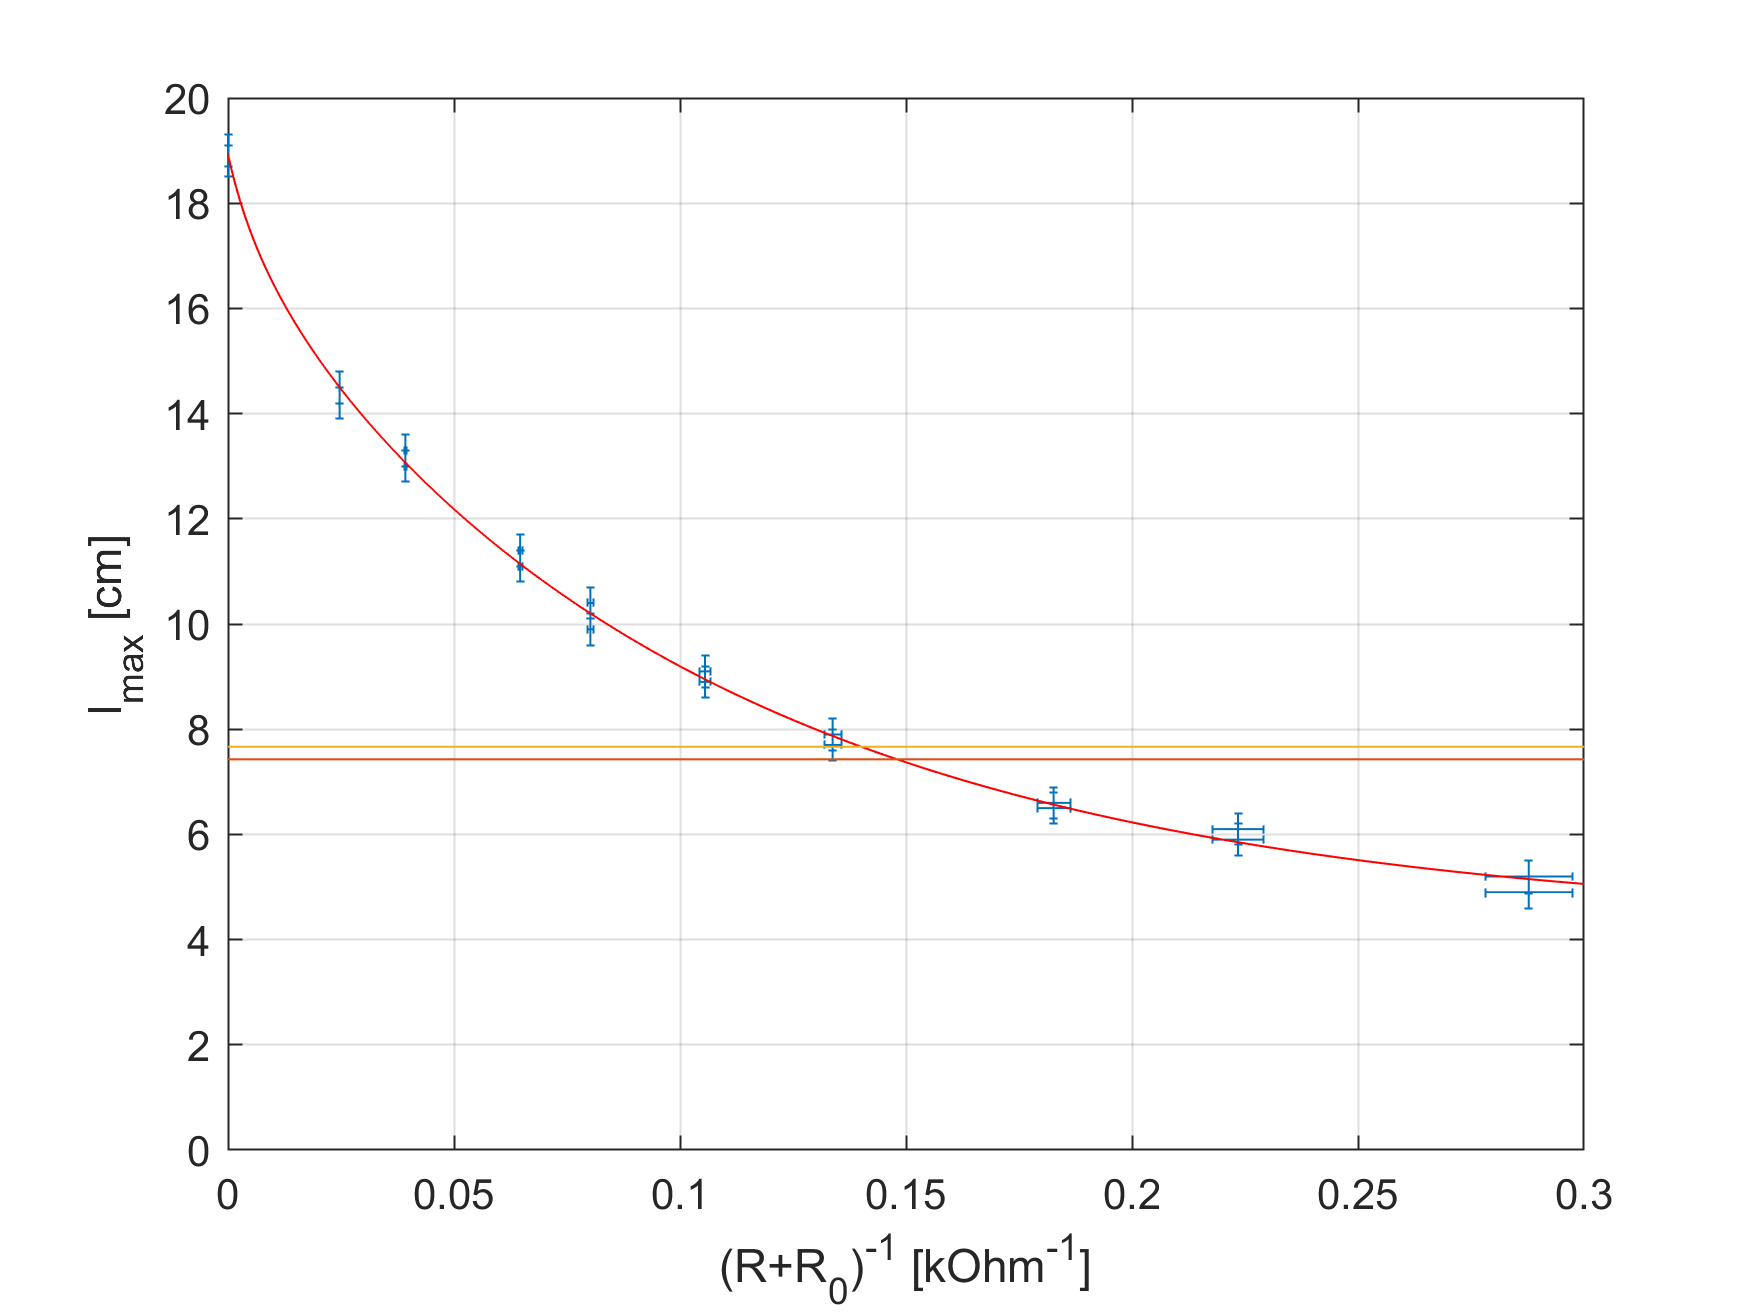
\includegraphics[width=12cm]{PlotC.png} 
   \caption{Зависимость максимального отклонения зайчика $l_{max}$ от шунтирующего сопротивления $R$  в баллистическом режиме работы гальванометра.} 
   \label{PlotC} 
   \end{figure}
   
Известно, что в критическом режиме $l_{max}$ в $e$ раз меньше, чем при незатухающих колебаниях. $l_{max \text{ незатухающих}}$ для незатухающих колебаний рассчитывается как $l_{max \text{ незатухающих}} = l_{max}(R=0)\exp^{\theta_0/4}$. Интервал значений в которые должно попадать $l_{max \text{ крит}}$ представлен на том же графике. Получая координаты пересечения нашей зависимости с этим интервалом можно найти $R_\text{кр}$. Полученное значение $(R_\text{кр} + R_0)^{-1} = [0.143 \pm 0.010] kOhm^{-1}$, откуда значение  \textbf{$R_\text{кр} = [6.5 \pm 0.5] kOhm$}.

Видно, что были получены три довольно разных значений $R_\text{кр}$:\medskip

$R_\text{кр} \approx 9.2 kOhm$ получено подбором,\medskip

$R_\text{кр} =  [10.9 \pm 0.5]kOhm$ получено в стационарном режиме,\medskip

$R_\text{кр} = [6.5 \pm 0.5] kOhm$ получено в баллистическом режиме.\medskip

Эксперименты других исследователей нашего потока дают такие же несовпадающие значения  $R_\text{кр}$.

Где же ошибка? Когда всё пошло не так?

*возвращается из пространных мыслей о том, что пошло не так*\medskip

Было получено значение \textbf{$C_{Q\text{ кр}} = 2a \frac{R_1}{R_2}\frac{U_0C}{l_{max \text{ крит}}} = [2.09 \pm 0.11]*10^{-6}C$} ( здесь $\frac{R_1}{R_2} = 1/70$, а $l_{max \text{ крит}} = [7.55 \pm 0.12]cm$).


\bigskip

\subsection*{Итог}
\bigskip

Гальванометр исследован. Получены значения его динамической $C_1 = [0.601 \pm 0.14] \mu A$ и баллистической $C_{Q\text{ кр}} = [2.09 \pm 0.11]*10^{-6}C$ постоянных. Также были получены значения $R_\text{кр}$ тремя разными способами:\medskip

$R_\text{кр} \approx 9.2 kOhm$ получено подбором,\medskip

$R_\text{кр} =  [10.9 \pm 0.5]kOhm$ получено в стационарном режиме,\medskip

$R_\text{кр} = [6.5 \pm 0.5] kOhm$ получено в баллистическом режиме.\medskip

\subsection*{Планы на будущее}
\bigskip

Разобраться, почему такие различия в значениях $R_\text{кр}$, полученных разными способами.
 
\end{document} % конец документа